%% Based on techreport.tex template as sent by Erik Burger on 2023-11-20
%% 
%% Karlsruhe Institute of Technology
%% Institute for Program Structures and Data Organization
%% Chair for Software Design and Quality (SDQ)
%%
%% Dr.-Ing. Erik Burger
%% burger@kit.edu
%%
%% S ee https://sdq.kastel.kit.edu/wiki/Dokumentvorlagen
%%
%% Version 1.0, 2023-11-20

%% Available page modes: oneside, twoside
%% Available languages: english, ngerman
%% Available modes: draft, final (see README)
\documentclass[oneside, ngerman]{sdqtechreport}

%% ---------------------------------
%% | Information about the document |
%% ---------------------------------

%% Name of the group and authors
\author{von Neptun - \\
Paul Buda, Martin Scheuermann, Stephan Schneider, \\
Simon Schütz und Nils Seibert}

%% Title (and possibly subtitle) of the thesis
\title{Pflichtenheft}

\subtitle{zur Android-App Neptune}

%% You can put a logo in the ``logos'' directory and include it here
%% instead of the SDQ logo
% \grouplogo{myfile}
%% Alternatively, you can disable the group logo
% \nogrouplogo

\date{01.12.2023}

%% For example texts -- please remove in the final version
\usepackage{blindtext}

%% ====================================
%% ====================================
%% ||                                ||
%% || Beginning of the main document ||
%% ||                                ||
%% ====================================
%% ====================================
\begin{document}

%% Set PDF metadata
\setpdf

%% Set the title
\maketitle

%% ------------------------
%% |   Table of Contents  |
%% ------------------------
\tableofcontents

%% -----------------
%% |   Main part   |
%% -----------------
\cleardoublepage

%% -------------------
%% | Example content |
%% -------------------

\chapter{Einleitung}
\label{chap:Einleitung}

\section{Einführung}
\label{sec:Einleitung:Einführung}
Musik spielt im Leben vieler Menschen eine enorm wichtige Rolle. Insbesondere bei Partys und Zusammenkünften mit Freunden sorgt eine gute Musikauswahl für eine gute Stimmung unter den Anwesenden. Aber auch der umgekehrte Fall ist vielen sicherlich gut bekannt – gefällt die abgespielte Musik den Anwesenden nicht, so kann dies die Stimmung erheblich trüben.

Nahezu alle der heute gängigen Musikstreaming-Anbieter versuchen bereits mit proprietären Lösungen, dem entgegenzuwirken. In der Praxis jedoch sind die eigens von den Anbietern angebotenen Lösungen häufig nicht praktikabel. Die Ursachen hierfür sind divers, so setzen die von den Anbietern selbst entwickelten Tools häufig voraus, dass alle Teilnehmer über ein bestehendes Abonnement beim entsprechenden Anbieter verfügen. 

Das Ziel des Projekts „Neptune“ ist es, eine praktikable Lösung für die eingangs beschriebene Problematik anzugeben. Hierzu soll im Rahmen des Moduls „Praxis der Softwareentwicklung“ eine Android-App entwickelt werden, mithilfe derer über die bei einer Party oder einem vergleichbaren Event abgespielte Musik entschieden werden kann.

Hierzu sollen die Anwesenden in verschiedenen verfügbaren Abstimmungs-Modi Musikvorschläge einbringen und über diese abstimmen können. Die Musik soll dann über das Endgerät einer weiteren anwesenden Person, des sogenannten „Hosts“, abgespielt werden. 
Mittels der Einbindung eines gängigen Musikstreaming-Service soll die App in die Lage versetzt werden, einen breiten Musikkatalog bereitzustellen.


\section{Anwendungsbereich}
\label{sec:Einleitung:Anwendungsbereich}

Das Ziel von Neptune ist es, die Musikauswahl bei privaten Veranstaltungen, wie zum Beispiel studentische WG- und Wohnheimpartys, einfacher und gerechter zu gestalten.
Die Android-App Neptune bietet Gruppen die Möglichkeit jeden an der Musikauswahl zu beteiligen und über die Abspielreihenfolge demokratisch abzustimmen. Durch die Integration mit einem Audio-Streaming-Dienst wie Spotify kann Neptune automatisch die am besten bewerteten Songs abspielen. Damit ist es möglich Songwünsche von Gästen zu erfüllen, ohne einen "DJ"  der die Wünsche entgegen nimmt und sie manuell in die Warteschlange hinzufügt.

Bei der Erstellung einer Listening-Session kann der Gastgeber die verfügbaren Lieder nach Belieben auf verschiedene Genres oder eine Playlist beschränken. Nach Auswahl des Modus kann der Gastgeber die Gäste einladen, sich an der Musikauswahl zu beteiligen, indem er einen sechsstelligen Zahlencode oder einen Link weitergibt. Die Gäste können dann in der App Lieder in die Abstimmungsliste hinzufügen und mit dem Verteilen von Likes Lieder in der Liste nach oben voten und sie somit schneller zum Abspielen bringen. Der Host hat durch eine Kontrollansicht einen Überblick über die Spotifywarteschlange, sowie die Abstimmungsliste in Neptune. 

Eine vollständige Beschreibung der Anwendungsfälle sind in den Use-Case-Diagrammen zu entnehmen   LINK


\section{Zielgruppe}
\label{sec:Einleitung:Zielgruppe}

Die primäre Zielgruppe von Neptune besteht aus Veranstaltern und Besuchern von Privatpartys, die zwischen 5-50 Besucher haben.  


\chapter{Zielbestimmungen}
\label{chap:Zielbestimmungen}

\section{Musskriterien}
\label{sec:Zielbestimmungen:Musskriterien}
\begin{itemize}
    \item ALLGEMEINES
    \item Nutzer der App können genau zwei verschiedene Rollen bekleiden. Diese verfügen über voneinander unterschiedliche Eigenschaften, welche je nach gewähltem Abstimmungsmodus variieren können (GENAUER BEGRIFFLICH DEFINIEREN)
    \begin{itemize}
        \item Host: Der Host erstellt das Event und fungiert als Administrator. Nur er kann Einladungen für weitere Teilnehmer generieren. Darüber hinaus kann nur er den Abstimmungsmodus auswählen.
        \item Teilnehmer: Teilnehmer können einem Event beitreten und basierend auf dem von dessen Host gewähltem Abstimmungsmodus über abzuspielende Musik abstimmen.
    \end{itemize}
    \item In der App stehen verschiedene Abstimmungsmodi mit unterschiedlichen Eigenschaften bereit (AUSARBEITEN)
    \begin{itemize}
        \item General Mode
        \item Playlist Mode
        \item Genre Mode
        \item Artist Mode
        \item ALLE SAUBERER AUSDEFINIEREN, oder darauf verweisen, oder halt nicht, von Stepahns Hochgeladenem nehmen
        \item Soll rein: Nicht-Spotify-Nutzer können nur abstimmen und nicht selbst vorschlagen.
    \end{itemize}
    \item In der App steht ein durchsuchbarer Musikkatalog zur Verfügung. (ÜBERABEITEN, der Katalog kommt per API...)
    \item 25 NUTZER THEMEATIK sauber definieren: Erstmal nur für 25 Nutzer zugelassen, bis Spotify das approved
    \item Die durch Abstimmung festgelegte Musik wird über externe Musikstreaming-Dienste abgespielt.
    \item Wurde ein Song abgespielt, so soll er innerhalb eines bei Einrichtung der Session festgelegten Intervalls kein zweites Mal abgespielt werden können (ÜBERARBEITEN, evt. mit Modus-Definition zusammenfügen)
    \item Sprachen: Englisch und deutsch (AUSFORMULIEREN)

\end{itemize}

\section{Wunschkriterien}
\label{sec:Zielbestimmungen:Wunschkriterien}
\begin{itemize}
    \item In der App sollen Statistiken bezüglich des Ablaufs eines Events zur Verfügung stehen. (LASSEN, oder SAUBER AUSDEFINIEREN) (MARTIN)
    \item Im Falle dessen, dass die Teilnehmer keine neue Musik vorschlagen und die Warteschlange hierdurch leer ist, soll die App mittels einer Autoplay-Funktion dennoch kontinuierlich Musik abspielen.

\end{itemize}

\section{Abgrenzungskriterien}
\label{sec:Zielbestimmungen:Abgrenzungskriterien}
\begin{itemize}
    \item Musik soll nicht innerhalb der App selbst abgespielt werden.
    \item Im Rahmen des Projekts soll keine öffentlich zugängliche API und insgesamt keine Schnittstelle für weitere externe Anwendungen bereitgestellt werden
    \item Die App soll, abgesehen von einer Internetverbindung, keine weiteren alternativen Netzwerktechnologien wie Bluetooth o.ä. nutzen.

\end{itemize}



\chapter{Anforderungen an die Produktumgebung}
\label{chap:Produktumgebung}

\section{Software}
\label{sec:Produktumgebung:Software}

\begin{itemize}
    \item Spotify API
    \item ...
\end{itemize}

\section{Hardware}
\label{sec:Produktumgebung:Hardware}

\begin{itemize}
    \item Smartphone mit mindestens Android 7.0
\end{itemize}



\chapter{Produktfunktionen}
\label{chap:Produktfunktionen}

\section{Grundfunktionen}
\label{sec:Produktfunktionen:Software}

\section{Erweiterte Funktionen}
\label{sec:Produktfunktionen:Hardware}



\chapter{Produktdaten}
\label{chap:Produktdaten}

\section{Systemdaten}
\label{sec:Produktdaten:Systemdaten}

Als Systemdaten werden sämtliche Daten zur Generierung der Benutzeroberfläche gespeichert, sowie Sitzungs-IDs oder Geräte-Tokens und Daten zum Auffinden des Servers. (Evt. kommen noch weiter hinzu wie Benutzereinstellungen, Historiendaten (einfachere Suche vllt.),  App-Zustandsdaten, ...)

\section{Nutzerdaten}
\label{sec:Produktdaten:Nutzerdaten}

Falls das Account-System nicht umgesetzt wird, werden keine sensiblen Nutzerdaten verarbeitet und gespeichert. Ausschließlich die zum Aufruf der Musik-App API benötigten Daten (WELCHE SIND DAS ???) sowie Sitzungs-IDs oder Geräte-Tokens werden verarbeitet und gespeichert.
Im Fall eines Account-Systems kommen Anmeldedaten, sowie weitere (optionale ???) persönliche Nutzerdaten hinzu.



\chapter{Systemmodell}
\label{chap:Systemmodell}

Es erfolgt eine Teilung in Client und Server, wobei auf dem Server der größte Teil der Logik geschieht.

Für den Client könnte eine Model-View-Controller-Architektur verwendet werden. Besonders relevant ist dabei, dass Anfragen an die Musik-API sinnvoll eingegliedert werden, da diese einen großen Teil des App-Umfangs ausmachen. Vermutlich würde man sowohl Musik-API als auch Kommunkation mit dem Server in den Bereich des Controllers einordnen.

Hier evt. noch Grafiken einfügen...



\chapter{Benutzeroberfläche}
\label{chap:Benutzeroberfläche}

\section{Einführung}
\label{sec:Benutzeroberfläche:Einführung}
\textbf{} Die Benutzeroberfläche wird so gestaltet, dass diese einfach von Nutzern ohne Vorkenntnissen über die App genutzt werden kann. 

\section{Startmenü}
\label{sec:Benutzeroberfläche:Startmenü}
Der Nutzer landet beim Start der App immer im Startmenü.

\section{Participant Ansicht}
\label{sec:Benutzeroberfläche:participantAnsicht}
In der Participant Ansicht kann der Nutzer einer Gruppe beitreten und je nach Modus neue Lieder vorschlagen und liken.

\section{Host Ansicht}
\label{sec:Benutzeroberfläche:hostAnsicht}
In der Host Ansicht kann der Host einen Modus auswählen und Einstellungen für die Session definieren. Des weiteren kann er wie ein Participant Lieder hinzufügen und liken. Zusätzlich kann der Host Lieder aus der Queue löschen und Lieder aus der Vorschlagsliste zur Queue hinzufügen

\section{Grafikentwürfe}
\label{sec:Benutzeroberfläche:Grafikentwürfe}

\begin{figure}
   \begin{minipage}[b]{.4\linewidth} % [b] => Ausrichtung an \caption
      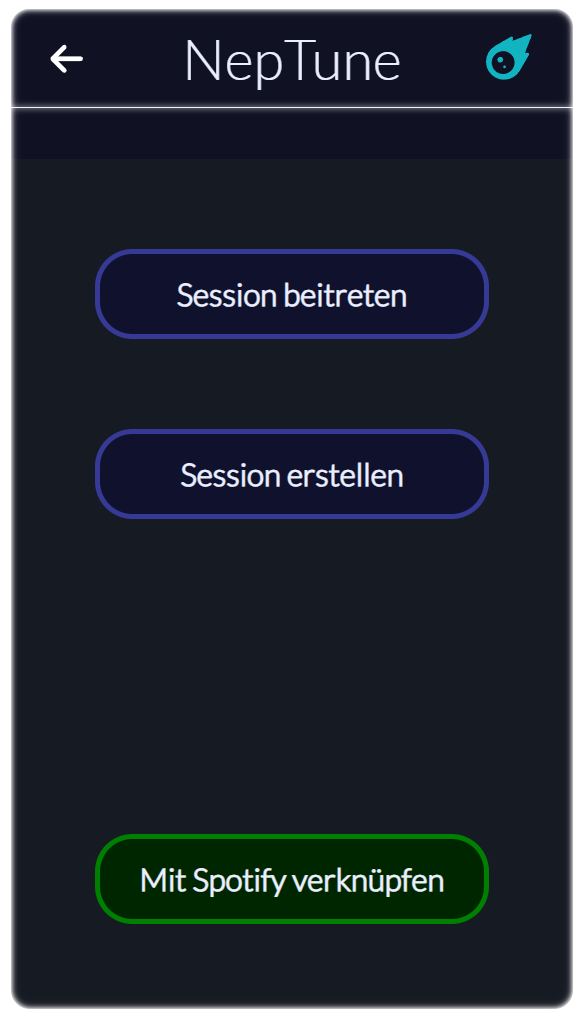
\includegraphics[width=5.5cm]{LATEX/Pflichtenheft/GraphicDesigns/startPage.png}
      \caption{startPage}
   \end{minipage}
   \hspace{2cm}% Abstand zwischen Bilder
   \begin{minipage}[b]{.4\linewidth} % [b] => Ausrichtung an \caption
      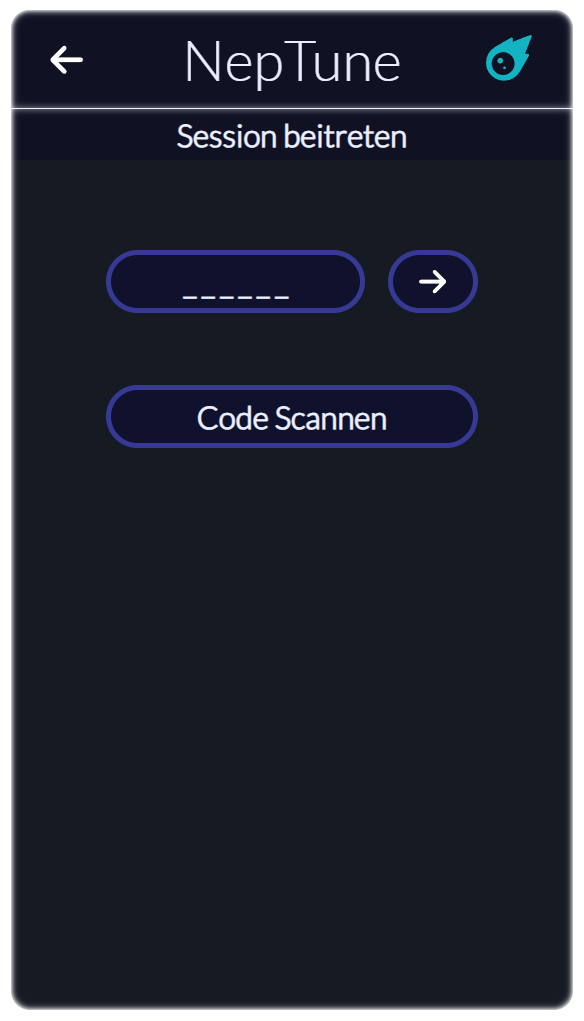
\includegraphics[width=5.5cm]{LATEX/Pflichtenheft/GraphicDesigns/userJoinGroupPage.png}
      \caption{userJoinGroupPage}
   \end{minipage}
   
   \begin{minipage}[b]{.4\linewidth} % [b] => Ausrichtung an \caption
      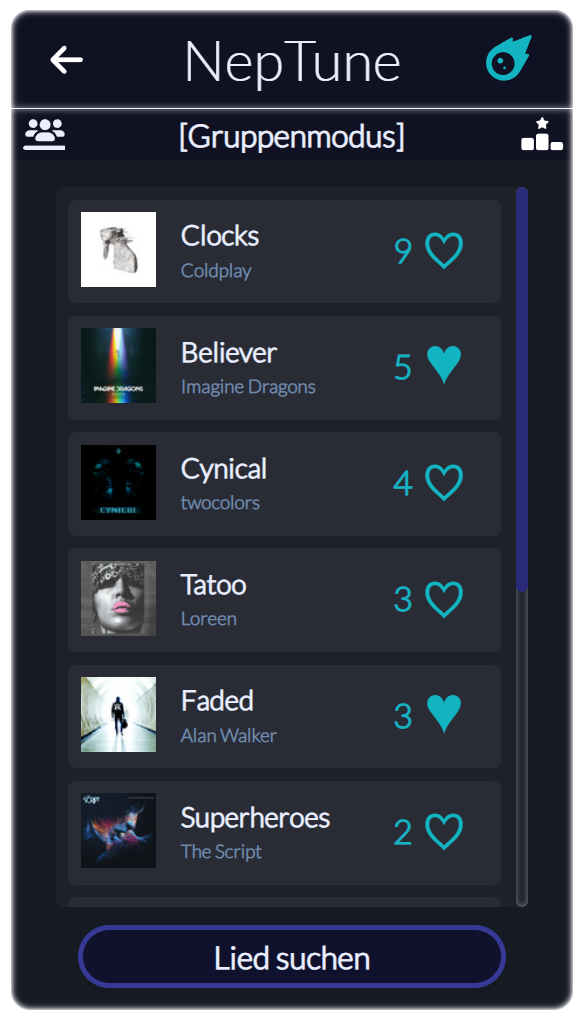
\includegraphics[width=5.5cm]{LATEX/Pflichtenheft/GraphicDesigns/userVotePage.png}
      \caption{userVotePage}
   \end{minipage}
   \hspace{2cm}% Abstand zwischen Bilder
   \begin{minipage}[b]{.4\linewidth} % [b] => Ausrichtung an \caption
      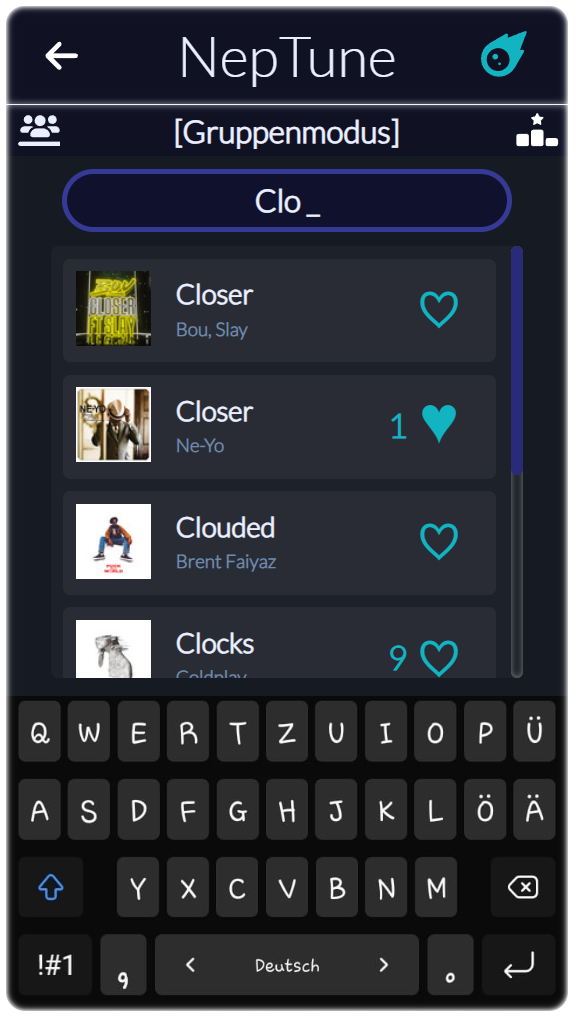
\includegraphics[width=5.5cm]{LATEX/Pflichtenheft/GraphicDesigns/userSearchPage.png}
      \caption{userSearchPage}
   \end{minipage}
\end{figure}

\begin{figure}
   \begin{minipage}[b]{.4\linewidth} % [b] => Ausrichtung an \caption
      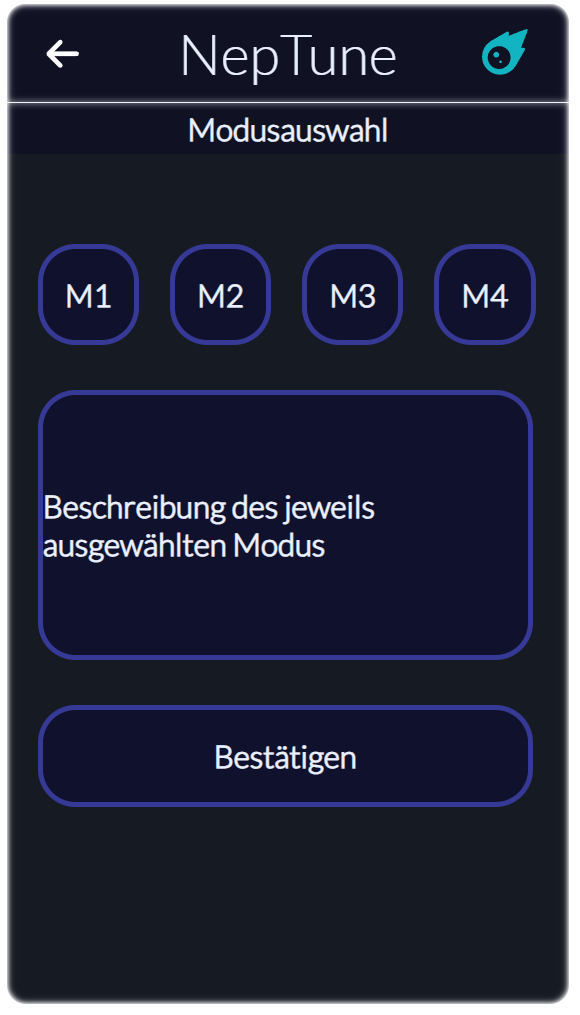
\includegraphics[width=5.5cm]{LATEX/Pflichtenheft/GraphicDesigns/hostModusSelectPage.png}
      \caption{hostModusSelectPage}
   \end{minipage}
   \hspace{2cm}% Abstand zwischen Bilder
   \begin{minipage}[b]{.4\linewidth} % [b] => Ausrichtung an \caption
      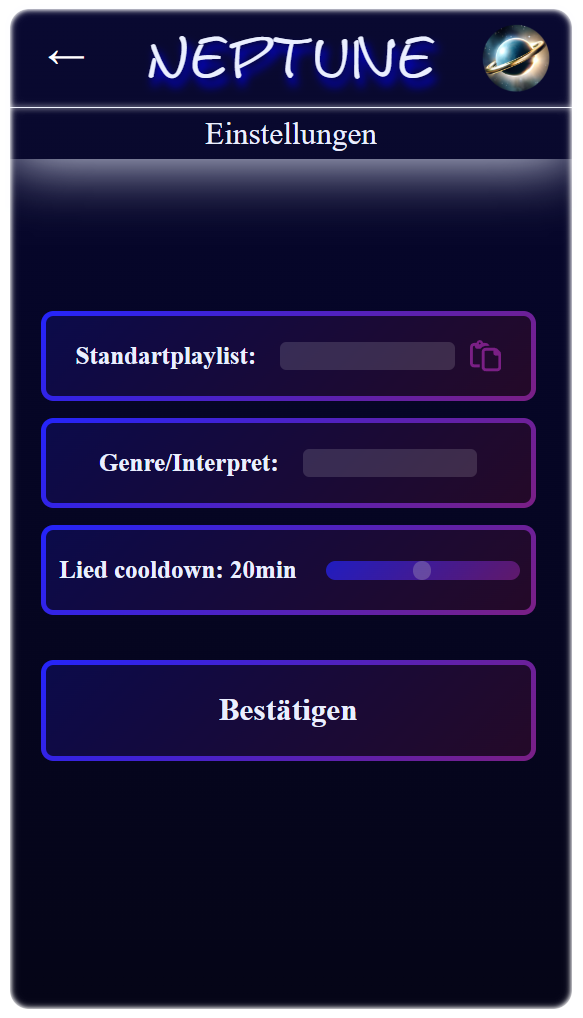
\includegraphics[width=5.5cm]{LATEX/Pflichtenheft/GraphicDesigns/hostModusSettingsPage.png}
      \caption{hostModusSettingsPage}
   \end{minipage}
   
   \begin{minipage}[b]{.4\linewidth} % [b] => Ausrichtung an \caption
      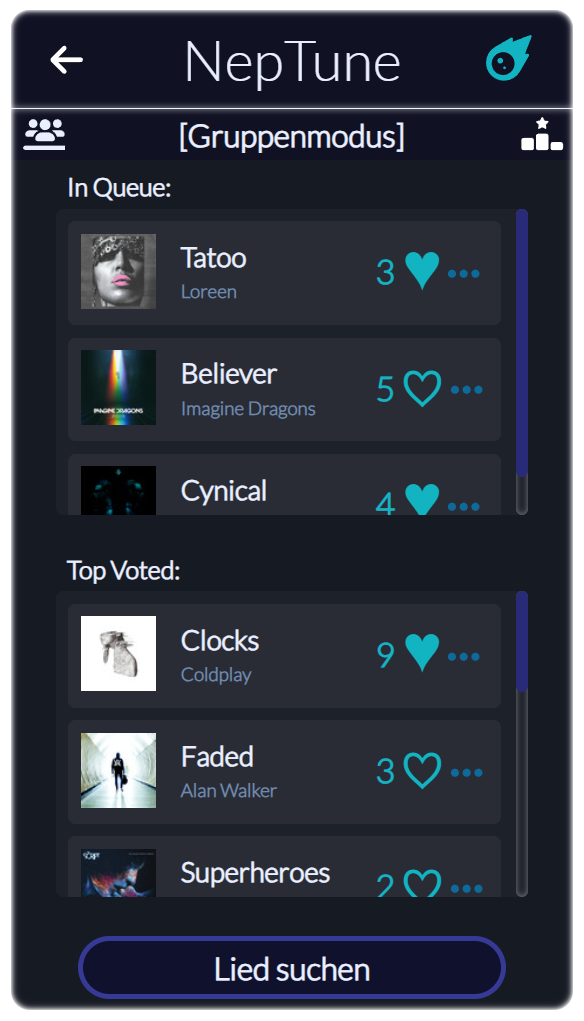
\includegraphics[width=5.5cm]{LATEX/Pflichtenheft/GraphicDesigns/hostControlPage.png}
      \caption{hostControlPage}
   \end{minipage}
   \hspace{2cm}% Abstand zwischen Bilder
   \begin{minipage}[b]{.4\linewidth} % [b] => Ausrichtung an \caption
      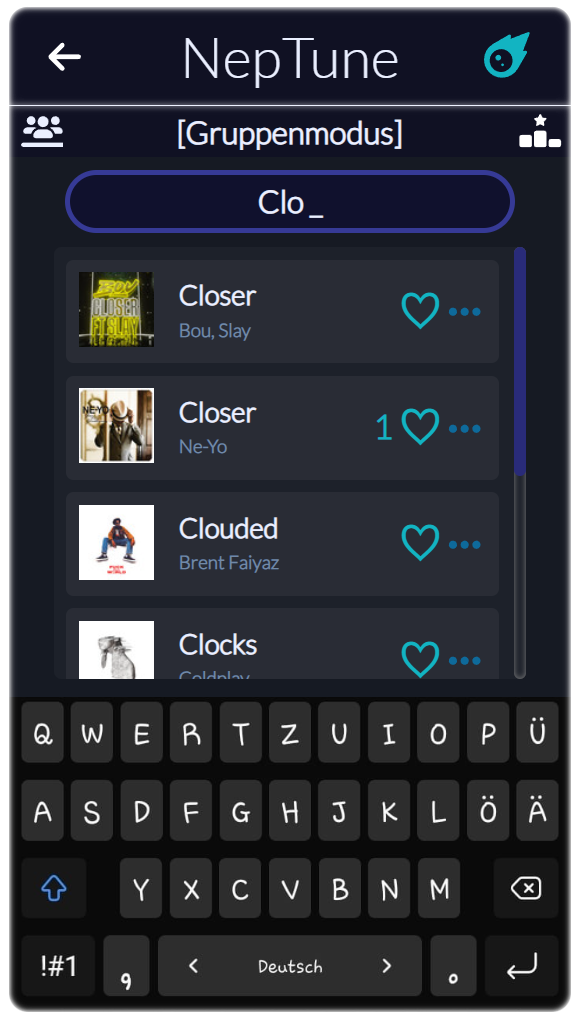
\includegraphics[width=5.5cm]{LATEX/Pflichtenheft/GraphicDesigns/hostSearchPage.png}
      \caption{hostSearchPage}
   \end{minipage}
\end{figure}

\begin{figure}
   \begin{minipage}[b]{.4\linewidth} % [b] => Ausrichtung an \caption
      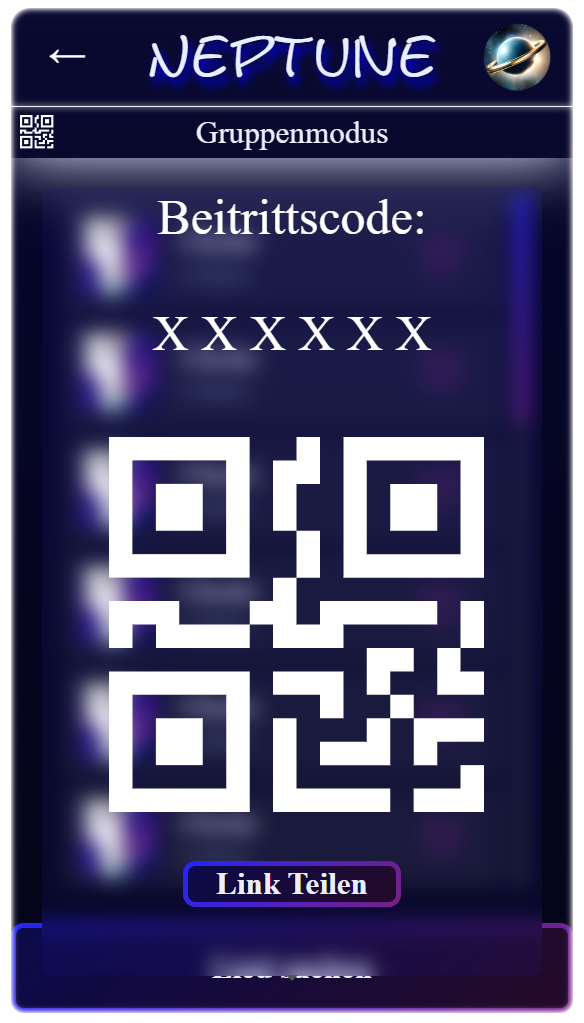
\includegraphics[width=5.5cm]{LATEX/Pflichtenheft/GraphicDesigns/shareLinkPopUpPage.png}
      \caption{shareLinkPopUpPage}
   \end{minipage}
   \hspace{2cm}% Abstand zwischen Bilder
   \begin{minipage}[b]{.4\linewidth} % [b] => Ausrichtung an \caption
      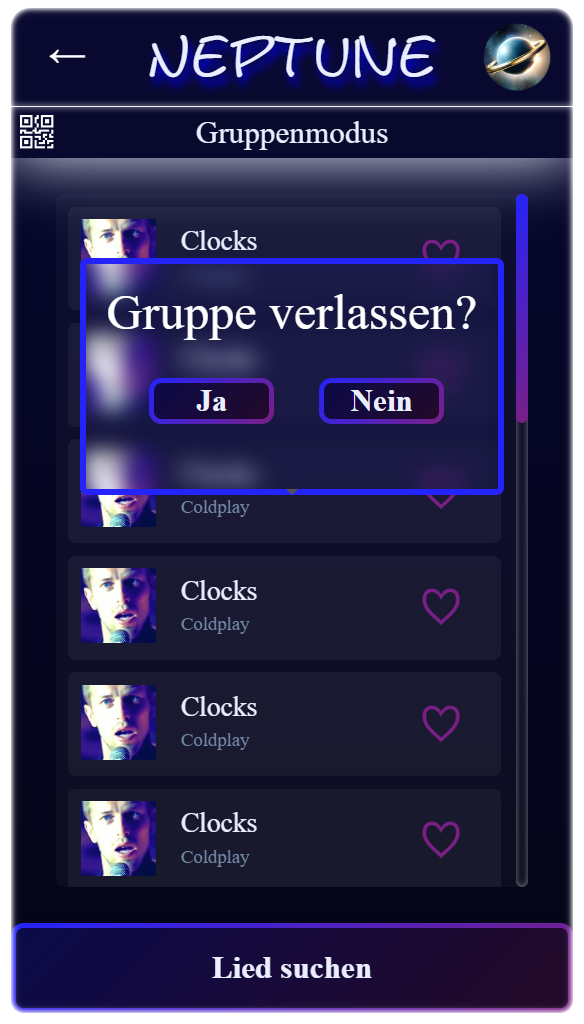
\includegraphics[width=5.5cm]{LATEX/Pflichtenheft/GraphicDesigns/userLeaveGroupPopupPage.png}
      \caption{userLeaveGroupPopupPage}
   \end{minipage}
   
   \begin{minipage}[b]{.4\linewidth} % [b] => Ausrichtung an \caption
      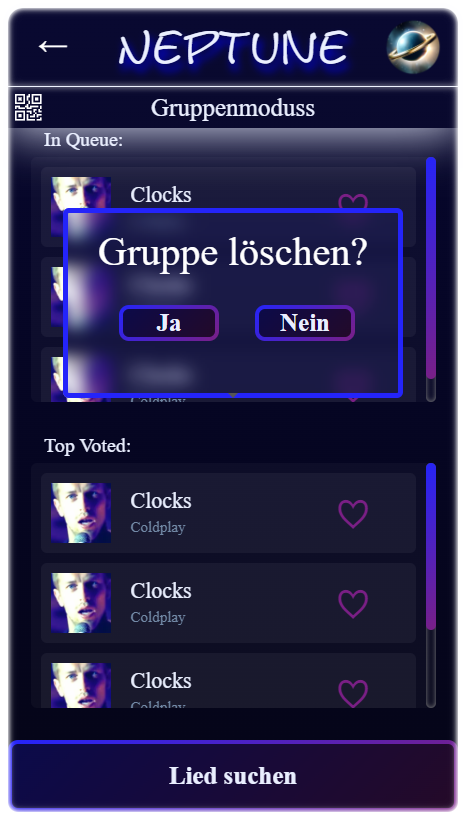
\includegraphics[width=5.5cm]{LATEX/Pflichtenheft/GraphicDesigns/hostDeleteGroupPopupPage.png}
      \caption{hostDeleteGroupPopupPage}
   \end{minipage}
\end{figure}

Spare Text:

Um ein übersichtliches Startmenü zu gewährleisten kann der Nutzer nur zwischen den Optionen "Gruppe beitreten" und "Gruppe erstellen" wählen. 

Im Startmenü kann der Nutzer entweder über die Buttons in der Mitte einer Gruppe beitreten, oder eine Gruppe erstellen. Über den Zurück-Knopf oben links verlässt der Nutzer die App.

Auf der Nutzer Abstimmungsseite sieht der Nutzer lieder bereits von Gruppenmitglieder vorgeschlagen und geliked wurden. Zudem kann er Lieder liken, welche er noch nicht geliked hat. Durch klicken des Lieder suchen Buttons gelangt der Nutzer zur Liedersuche. Über den Zurück-Knopf oben links gelangt der Nutzer zurück zum Startmenü. Dieser Vorgang muss über ein Pop-Up Fenster bestätigt werden, da gleichseitig die Gruppe verlassen wird.




\chapter{Qualitätszielbestimmungen}
\label{chap:Qualitätszielbestimmungen}

\textbf{Korrekte Funktionalität}: Die korrekte Funktionalität der App muss gewährleistet sein. Maßgeblich zur Definition dieser korrekten Funktionalität ist dieses Pflichtenheft und insbesondere die Musskriterien aus dem Kapitel der Zielbestimmungen (\ref{sec:Zielbestimmungen:Musskriterien}).

\textbf{Benutzerfreundlichkeit}: Die App soll eine einfache und intuitive Benutzererfahrung bieten. Die Navigation innerhalb der App soll für alle Benutzer leicht verständlich sein, ohne dass diese eine Einführung in die App-Bedienung benötigen.

\textbf{Schnelligkeit}: Die App soll durch Reaktionsschnelligkeit ein flüssiges und ansprechendes Nutzungserlebnis ermöglichen. Jede Schaltflächenbedienung soll eine unmittelbares Feedback für den Benutzer auslösen, ohne dass dieser eine Wartezeit bemerkt, solange das Endgerät hinreichend aktuell ist.

\textbf{Sicherheit der Benutzerdaten}: Es ist essentiell, dass die persönlichen Daten der Benutzer geschützt sind. Jegliche Interaktion mit und Datenverarbeitung durch die App muss datenschutzkonform sein und Datensicherheit bieten.

\textbf{Stabilität und Zuverlässigkeit}: Die App muss robust sein und selbst unter Last und bei mäßig vielen gleichzeitigen Benutzern stabil bleiben, sodass Abstürze oder unerwartete Fehler weitestgehend vermieden werden.

\textbf{Wartbarkeit und Portierungsmöglichkeiten}: Die Architektur der App soll gut wartbar sein, um zukünftige Anpassungen oder Erweiterungen zu ermöglichen. Zudem soll die Architektur die Möglichkeit zur verhältnismäßig einfachen Portierung der App auf andere mobile Betriebssysteme wie iOS bieten. 

\textbf{Grundsätzliches zur Qualität}: Diese Qualitätszielbestimmungen werden während allen Projektphasen beachtet und in der Qualitätssicherungsphase intern abgenommen. Die Qualität der App besitzt während allen Projektphasen einen sehr hohen Stellenwert: Sie wird stets als Priorität betrachtet und in der Qualitätssicherungsphase abschließend und eingehend geprüft.

GERICHTSFEST machen



\chapter{Anwendungsfälle}
\label{chap:Anwendungsfälle}



\chapter{Testfälle und -szenarien}
\label{chap:Tests}

In diesem Kapitel werden alle Testfälle und -szenarien definiert, die einen oder mehrere Benutzer des fertiggestellten Produkts durchgeführt werden. Die hier definierten Testfälle sollen deshalb explizit keine technischen Funktionalitäten testen, die ausreichend detailliert erst während der Entwurfsphase festgelegt werden. Solche technischen Funktionalitäten werden durch Unittests abgedeckt, die während der Entwurfs- und Implementierungsphase entworfen und implementiert werden.

\section{Testfälle}
\label{sec:Tests:Testfälle}

Testfälle sind Tests zu aus Benutzersicht atomaren Vorgängen. Jeder Testfall bezieht sich also auf eine einzelne atomare Benutzereingabe. Eine solche Benutzereingabe besteht entweder aus einem einzelnen Touch-Eingabe oder einer inhaltlich sehr stark zusammenhängenden Folge von Touch-Eingaben, die als atomar betrachtet wird.

\begin{itemize}
    \item Starten und Laden der App
    \item Verlassen der App
    \item Beenden der App
    \item Gruppenbeitritt beginnen
    \item Gruppenbeitritt verlassen
    \item Eingabe des Zugangscodes zum Gruppenbeitritt
    \item Veranlassen des tatsächlichen Gruppenbeitritts
    \item Verlassen der Gruppe
    \item Abstimmen für einen Song
    \item Öffnen der Songsuche
    \item Verlassen der Songsuche
    \item Suchen eines Songs
    \item Hinzufügen eines Songs
    \item Gruppenerstellung beginnen
    \item Gruppenerstellung verlassen (Modus-Eigenschaften)
    \item Auswählen des Modus (evt. noch nicht atomar genug)
    \item Bestätigung des Modus
    \item Gruppenerstellung verlassen (Modus-Details)
    \item Auswählen der Details des Modus
    \item Bestätigung der Details des Modus
    \item Gruppe löschen
    \item Lied abspielen
    \item .......?
\end{itemize}

\section{Testszenarien}
\label{sec:Tests:Testszenarien}

Testszenarien sind eine Folge von atomaren Testfällen, die beispielhaft eine Benutzerinteraktion durchspielen.

\subsection{Testszenario 1: Eine simple Benutzung}
\label{subsec:Tests:Testszenarien:1}
Zwei Nutzer, ein Host (H) und ein normaler Benutzer (N) (???), erstellen eine Gruppe, bzw. treten einer Gruppe bei, schlagen einen Song vor und spielen diesen ab.

\begin{itemize}
    \item Starten und Laden der App (H, N)
    \item Gruppenerstellung beginnen (H)
    \item Auswählen des Modus (H)
    \item Bestätigung des Modus (H)
    \item Auswählen der Details des Modus (H)
    \item Bestätigung der Details des Modus (H)
    \item Gruppenbeitritt beginnen (N)
    \item Eingabe des Zugangscodes zum Gruppenbeitritt (N)
    \item Veranlassen des tatsächlichen Gruppeneitritts (N)
    \item Öffnene der Songsuche (N)
    \item Suchen eines Songs (N)
    \item Hinzufügen eines Songs (N)
    \item Abstimmen für einen Song (N)
    \item Lied abspielen (H)
    \item Verlassen der App (H, N)
\end{itemize}



\chapter{Entwicklungsumgebung}
\label{chap:Entwicklungsumgebung}

\section{Software}
\label{sec:Entwicklungsumgebung:Software}

\begin{itemize}
    \item Entwicklung
    \begin{itemize}
        \item Android Studio Giraffe (2022.3.1)
    \end{itemize}
    
    \item Versionsverwaltung
    \begin{itemize}
        \item GitHub
    \end{itemize}

    \item Modellierung
    \begin{itemize}
        \item Creately
    \end{itemize}

    \item Sonstige Software
    \begin{itemize}
        \item LATEX (Dokumentation)
        \item ...
    \end{itemize}
    
\end{itemize}

\section{Hardware}
\label{sec:Entwicklungsumgebung:Hardware}

\begin{itemize}
    \item Diverse Standard PCs
    \item Diverse Android Smartphones mit mindestens Android 7.0
\end{itemize}


\chapter{Begriffserklärungen}
\label{chap:Begriffserklärungen}

System: Gesamtes System, das entwickelt wird (App und Server)

App: Nur das, was auf dem Handy läuft

Server: Alles, was extern auf dem Server abgewickelt wird / entwickelt wird

Session: Eine Gruppe, von einem Host erstellt, mit der Musik vorgeschlagen und abgespielt wird

Host: Ersteller der Session, verwaltet Session, spielt die Musik ab

Participant: Teilnehmer einer Session (nicht der Host)

User: Participant oder Host

Queue: In der Queue befinden sich die Lieder, welche als nächstes gespielt werden

Vorschlagsliste: Die Vorschlagsliste enthält alle Lieder welche von einem User vorgeschlagen wurden


TODO: Produktleistungen weg, Anwendungsfälle vor Tests, Kapitel 3 mit 1 mergen und Betriebsbedingungen streichen, Produktumgebung evt. überarbeiten zu Betriebsbedingugen/Anforderungen, Produktfunktionen mit den Tests mergen.
\section{}
\end{document}
